\documentclass[a4paper]{article}

\usepackage[UTF8]{ctex}
\usepackage[a4paper,margin=1in]{geometry}
\usepackage{graphicx}
\usepackage{float}
\usepackage{listings}
\usepackage{booktabs}
\usepackage{color}
\usepackage{indentfirst}
\setlength{\parindent}{2em}
\usepackage{zhnumber}
\usepackage{adjustbox}
\usepackage{subcaption}
\usepackage{amsmath}
\usepackage{amssymb}
\usepackage{enumitem}
\usepackage{lmodern}
\usepackage{inconsolata}
\usepackage{multirow}
\usepackage{tikz}
\usetikzlibrary{positioning}
\usepackage{fancyhdr}
\usepackage{hyperref}

% 配置lstlisting支持中文
\lstset{
    language=C,
    basicstyle=\footnotesize\ttfamily,
    breaklines=true,
    keywordstyle=\bfseries\color{blue},
    commentstyle=\itshape\color{green!50!black},
    stringstyle=\bfseries\color{red},
    numbers=left,
    numberstyle=\tiny\color{gray},
    frame=single,
    backgroundcolor=\color{gray!5},
    showstringspaces=false,
    keepspaces=true,
    tabsize=4,
    extendedchars=true,
    inputencoding=utf8,
    literate={，}{{\textcolor{green!50!black}{，}}}{1}
             {。}{{\textcolor{green!50!black}{。}}}{1}
             {：}{{\textcolor{green!50!black}{：}}}{1}
             {；}{{\textcolor{green!50!black}{；}}}{1}
             {（}{{\textcolor{green!50!black}{（}}}{1}
             {）}{{\textcolor{green!50!black}{）}}}{1}
             {【}{{\textcolor{green!50!black}{【}}}{1}
             {】}{{\textcolor{green!50!black}{】}}}{1}
}

\newcommand{\projname}{计算机网络实验|实验八}
\newcommand{\reporttitle}{OSPF协议实验个人报告}
\newcommand{\groupno}{第一组}
\newcommand{\authorname}{马福泉}
\newcommand{\major}{计算机科学与技术}
\newcommand{\adviser}{谢逸}
\newcommand{\startdate}{2025年11月27日}
\newcommand{\labenddate}{2025年12月7日}
\newcommand{\labroom}{实验D402}

\pagestyle{fancy}
\fancyhf{}
\fancyhead[L]{\kaishu \projname}
\fancyhead[C]{\kaishu \reporttitle}
\fancyhead[R]{\kaishu \authorname}
\fancyfoot[C]{第 \thepage 页}
\renewcommand{\headrulewidth}{0.4pt}
\renewcommand{\footrulewidth}{0pt}


\begin{document}

% 封面
\begin{titlepage}
    \centering
    
\includegraphics[width=10cm]{img/SYSULogo.png}
    \vspace{1em}
    % 修改为换行并居中
    \par
    {\Large \kaishu
        \par
        \projname
        \par
    }
    \vspace{3em}
    {\fontsize{40pt}{42pt}\kaishu \selectfont \boldmath \reporttitle\par}
    \vspace*{\fill}
    \begin{center}
    {\Large
    \makebox[5em][s]{姓名}:\underline{\makebox[15em][c]{\kaishu 马福泉}}\\[1em]
    \makebox[5em][s]{学号}:\underline{\makebox[15em][c]{\kaishu 23336179}}\\[1em]
    \makebox[5em][s]{小组编号}:\underline{\makebox[15em][c]{\kaishu \groupno}}\\[1em]
    \makebox[5em][s]{专业}:\underline{\makebox[15em][c]{\kaishu \major}}\\[1em]
    \makebox[5em][s]{课程教师}:\underline{\makebox[15em][c]{\kaishu \adviser}}\\[1em]
    \makebox[5em][s]{起始日期}:\underline{\makebox[15em][c]{\kaishu \startdate}}\\[1em]
    \makebox[5em][s]{结束日期}:\underline{\makebox[15em][c]{\kaishu \labenddate}}\\[1em]
    \makebox[5em][s]{实验地点}:\underline{\makebox[15em][c]{\kaishu \labroom}}
    }
    \end{center}
    \vspace*{\fill}
\end{titlepage}

\section{承担的工作}

本次OSPF协议分析与配置实验，我参与了基础实验及拓展实验1、2的各个环节以及拓展实验3的方案探索与尝试，主要的工作如下：

\begin{enumerate}
    \item \textbf{实验环境搭建与物理连接}：协助队友根据实验要求设计基础拓扑（见图\ref{fig:topo}），完成路由器和主机的物理布线。核对端口连接，确保每一根网线都与正确设备接口相连，确保所有设备正常可访问。
\begin{figure}[h]
    \centering
    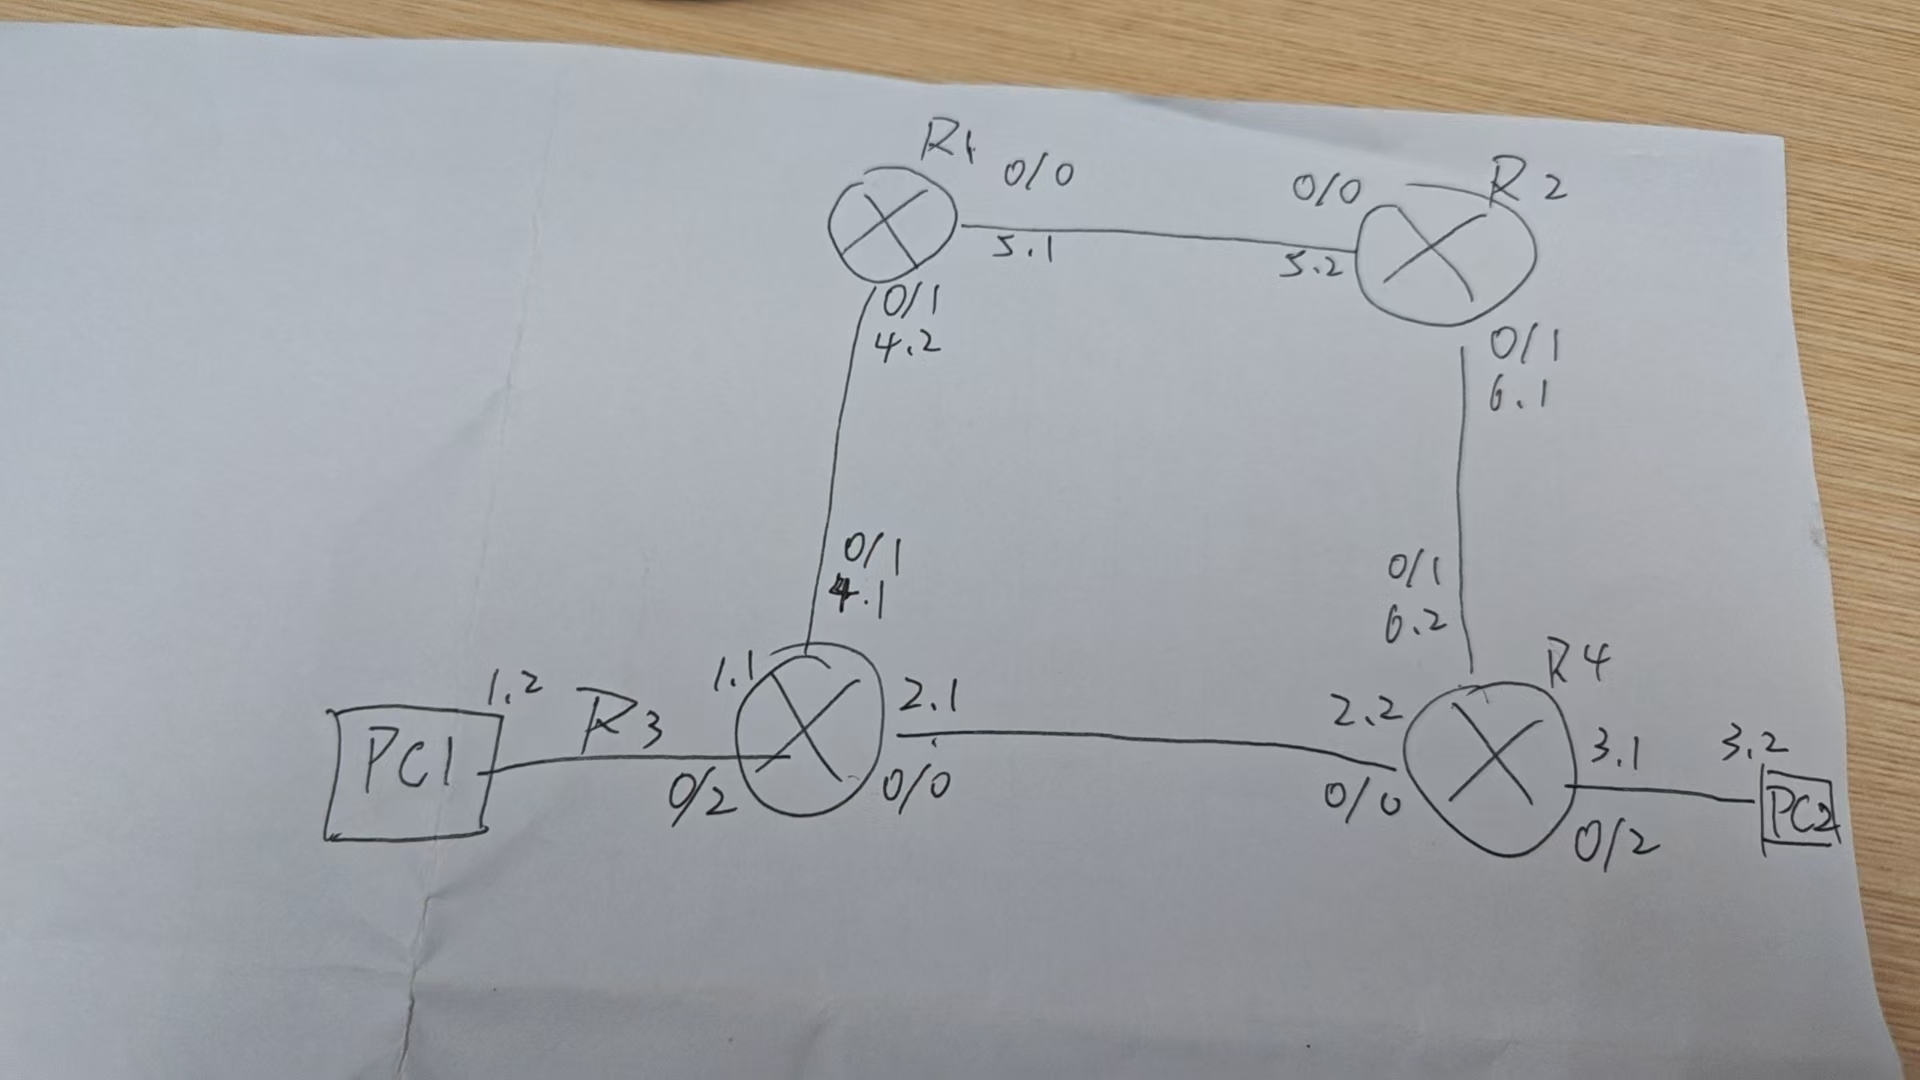
\includegraphics[width=0.8\textwidth]{img/1.jpg}
    \caption{拓扑图草稿}
    \label{fig:topo}
\end{figure}

    \item \textbf{基础OSPF配置与验证（单区域）}：
    \begin{itemize}
        \item 负责路由器OSPF协议的启用与网段宣告，例如在R1上执行如下配置：
\begin{lstlisting}
ospf 1 router-id 1.1.1.1
area 0
network 192.168.1.0 0.0.0.255
network 192.168.2.0 0.0.0.255
\end{lstlisting}
        \item 参与DR/BDR选举机制的验证，通过断开链路观察DR/BDR角色的变化，并记录相关现象。
        \item 协助完成拓扑扩展，在路由器上增加主机，验证新拓扑下的全网连通性。
    \end{itemize}

    \item \textbf{协议报文捕获与分析}：利用端口镜像和Wireshark软件捕获OSPF交互报文。
    \begin{itemize}
        \item 配置端口镜像命令，将流量复制到观察端口
        \item 详细分析OSPF头部结构，对比不同类型报文（Hello, DD, LSR, LSU, LSAck）的功能与字段含义。
    \end{itemize}

    \item \textbf{拓展实验1：OSPF认证与链路故障模拟}：
    \begin{itemize}
        \item 协助队友按环形拓扑配置全网OSPF，并添加路由器间的认证配置，确保安全性。
        \item 模拟R3与R4链路断开故障，使用\texttt{tracert}命令观察数据传输路径从直连切换为绕行骨干环路，验证OSPF的动态路由。
    \end{itemize}

    \item \textbf{拓展实验2：多区域OSPF配置}：
    \begin{itemize}
        \item 按多区域拓扑实施划分，配置区域边界路由器（ABR）。例如在R3上撤销原Area 0宣告并重新划分区域：
\begin{lstlisting}
undo network 192.168.4.0 0.0.0.255
area 1
network 192.168.4.0 0.0.0.255
\end{lstlisting}
        \item 捕获并分析跨区域的路由交换报文，验证区域间路由汇总机制。
    \end{itemize}

    \item \textbf{拓展实验3：特定路径控制的探索与尝试}：
    \begin{itemize}
        \item \textbf{方案设计与尝试}：尝试通过调整链路或连接隔壁组交换机来实现特定路径控制。
        \item \textbf{遇到的问题}：实验过程中已经观察路由表和配置静态路由和调整物理连接，发现路由正确，但是不知道为何数据包无法正常发送。
        \item \textbf{排查与结论}：虽然尝试了手动添加静态路由，但受限于设备环境，最终未能实现预期效果。
    \end{itemize}

    \item \textbf{实验总结与文档撰写}：整理实验截图、抓包数据及命令行输出。撰写个人心得体会。
\end{enumerate}

\section{遇到的困难及解决方法}

实验过程中遇到多项实际问题：

\begin{enumerate}
    \item \textbf{OSPF邻居关系未建立}
    
    \textbf{现象}：配置OSPF后，\texttt{show ip ospf neighbor}无邻居，\texttt{show ip ospf interface}发现接口未加入OSPF。
    
    \textbf{排查与解决}：检查network命令，发现反掩码写错，原为：
    \begin{lstlisting}
    network 192.168.1.0 255.255.255.0 area 0
    \end{lstlisting}
    正确应为：
    \begin{lstlisting}
    network 192.168.1.0 0.0.0.255 area 0
    \end{lstlisting}
    修改后邻居关系建立，控制台出现\texttt{OSPF-5-ADJCHANGE}日志。
    
    \item \textbf{接口未激活导致链路不通}
    
    \textbf{现象}：接口配置无误但无法ping通，\texttt{show ip interface brief}显示接口为\texttt{administratively down}。
    
    \textbf{解决}：进入接口模式执行\texttt{no shutdown}，接口状态变为\texttt{up/up}，链路恢复。
    
    \item \textbf{无法捕获OSPF建立过程报文}
    
    \textbf{现象}：在网络稳定状态下进行抓包，Wireshark仅能捕获到Hello报文，无法观察到DD、LSR、LSU及LSAck等邻居建立过程中的关键报文，无法完成协议头部分析。
    
    \textbf{排查与解决}：
    \begin{itemize}
        \item \textbf{尝试重置进程}：尝试在用户视图下使用\texttt{reset ospf process}命令重置OSPF进程：
\begin{lstlisting}
<R1> reset ospf process
\end{lstlisting}
        但因视图模式混淆（用户视图\texttt{<R1>}与系统视图\texttt{[R1]}）或模拟器指令支持问题，提示无法识别指令。
        
        \item \textbf{最终方案（重启接口）}：采用重启接口法强制邻居重新建立。进入连接邻居的接口视图（如G0/0/1），执行\texttt{shutdown}关闭接口，待邻居关系断开后，再执行\texttt{undo shutdown}：
\begin{lstlisting}
[R1] interface GigabitEthernet 0/0/1
[R1-GigabitEthernet0/0/1] shutdown
# 等待几秒，观察到邻居Down
[R1-GigabitEthernet0/0/1] undo shutdown
\end{lstlisting}
        此操作强制OSPF重新建立邻居关系，成功捕获到了完整的OSPF建连报文序列。
    \end{itemize}
\end{enumerate}

\section{体会与总结}

本次实验让我对OSPF协议的原理与实际配置有了系统、深入的理解：

\begin{itemize}
    \item \textbf{理论与实践结合}：通过实际配置和抓包，直观理解了OSPF的LSA泛洪、邻居建立、路由收敛等机制，理论知识得到了实践印证。
    \item \textbf{排错能力提升}：多次遇到配置、连通性等问题，学会了利用\texttt{show}、\texttt{debug}等命令逐步定位问题，查阅官方文档和资料，提升了独立排查和解决问题的能力。
    \item \textbf{对OSPF高级特性的理解}：通过多区域、路径控制等拓展实验，理解了OSPF区域划分、ABR、Cost等高级特性及其实际应用场景。
\end{itemize}

\end{document}
